\section{Daten verwalten in einer Datenbank} 
Wie wir im vergangenen Kapitel gesehen haben, ist Tabellenkalkulation-Software sehr gut dafür geeignet, Daten zu verwalten und zu untersuchen. Allerdings gibt es auch Einschränkungen. Zum Beispiel:
\begin{itemize}
  \item Die Anzahl Datensätze, die von einem Tabellenkalkulation-Programm verwaltet werden können ist limitiert: In Excel 2024 sind es 1'048'576 Zeilen. Das ist zwar viel, für die Verwaltung einer Social Media Plattform aber deutlich zu wenig.
  \item Später werden wir für die Social Media Plattform eine neue Tabelle \enquote{photos} einführen. Diese Tabelle wird mit der bereits bekannten Tabelle \enquote{users} verknüpft. Diese Verknüpfung lässt sich in einer Tabellenkalkulation nicht abbilden.
\end{itemize}

Eine der verbreitetsten Arten, Tabellen und Datenbanken zu erstellen, zu verändern und zu analysieren ist die Programmiersprache \gls{SQL} (\enquote{Strukturierte Abfrage-Sprache}). 
Im Folgenden verwenden wir die Datenbanken aus der Lern-Plattform InstaHub, um uns mit \gls{SQL}  vertraut zu machen. Dabei richten wir unser Augenmerk vorerst auf die Befehle, mit denen man wie in Excel die Daten filtern und sortieren kann.

\subsection{Einzelne Tabellen filtern und ordnen mit \texorpdfstring{\gls{SQL}}{SQL}}

\lstset{style=sql}

\subsubsection*{Syntax}
Die Sprache \acrfull{SQL} besteht, wie wir sehen werden, aus verschiedenen Schlüsselwörtern, wie etwa \lstinline|SELECT|, \lstinline|WHERE|, \lstinline|GROUP BY|, \lstinline|ORDER BY| usw. Dazu gibt es Folgendes zu beachten:
\begin{itemize}
  \item Ob wir diese Schlüsselwörter gross oder klein schreiben, spielt keine Rolle. Allerdings wird empfohlen, die Schlüsselwörter immer in Grossbuchstaben zu schreiben, um sie von Kolonnen-Namen, Tabellen-Namen usw. abzugrenzen.
  \item Wir können alle \gls{SQL}-Befehle auf einer einzigen Zeile schreiben, dadurch wird der Code aber deutlich weniger lesbar. Stattdessen empfiehlt es sich, vor gewissen Schlüsselwörtern wie \lstinline|SELECT|, \lstinline|WHERE| oder \lstinline|GROUP BY| eine neue Zeile zu erstellen. Dazu lohnt es sich, die Beispiele genau anzuschauen.
\end{itemize}

% \textbf{Kommentare} können in \gls{SQL}  auf zwei Arten geschrieben werden:

% \begin{lstlisting}
% -- 1. Kommentar auf einer Zeile
% /* 2. Kommentar über
% mehrere Zeilen */
% \end{lstlisting}

% need to add "texorpdfstring" to avoid warnings
\subsubsection*{Einfache Selektion: \texorpdfstring{\lstinline|SELECT|}{SELECT}}

Mit dem Befehl \enquote{\lstinline|SELECT col1,col2,... FROM tablename|} können wir gewisse Spalten ($=$ Kolonnen) \lstinline|col1,col2,...| aus einer Tabelle mit dem Namen \lstinline|tablename| auswählen. Wir können statt den Spaltennamen auch einfach einen Stern (\texttt{*}) tippen, um alle Kolonnen einer Tabelle zu erhalten, d.h. die gesamte Tabelle.


\begin{myexample}
  Loggen Sie sich als AdministratorIn bei Ihrem Instahub ein. Sie können unter folgendem Menu-Punkt Ihre eigene Datenbank administrieren:

  \begin{figure}[H]
    \centering
    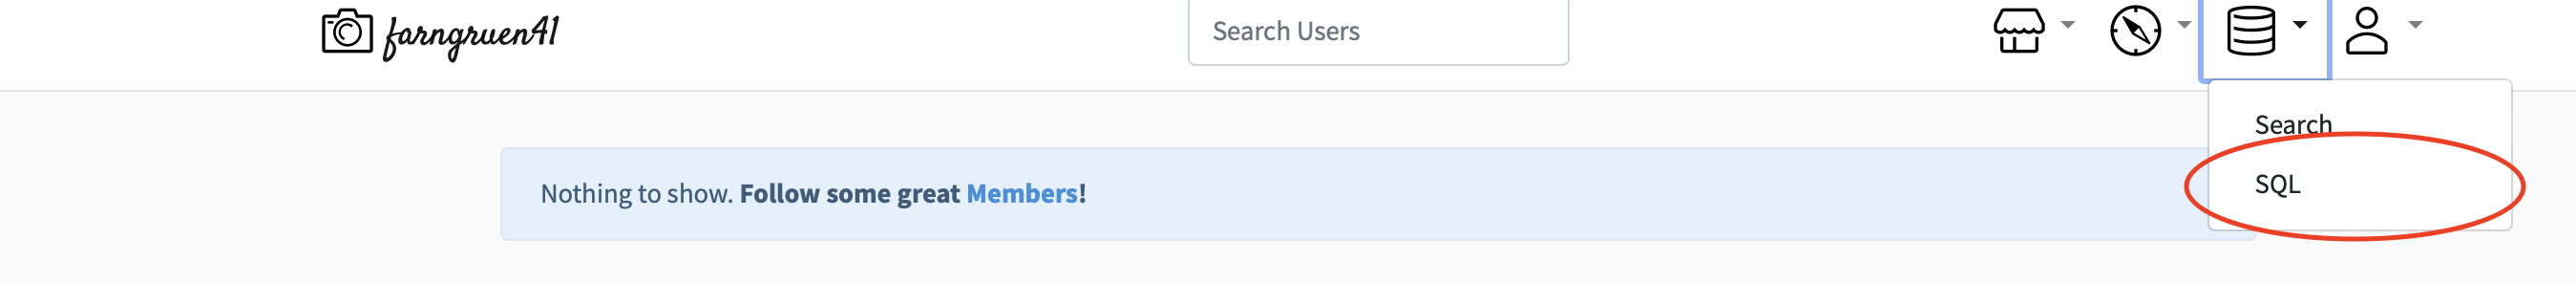
\includegraphics[width=.9\textwidth]{Grundlagen_Info/06_Datenbanken/Figures/instahub-SQL}
  \end{figure}

  % Als Erstes sehen Sie eine Liste der verfügbaren Tabellen sowie der dazugehörigen Spaltennamen (s. Bild unten).
  % Tabellennamen sind in \textcolor{orange}{Orange}, Spaltennamen in \green{grün} markiert.
  % \begin{figure}[H]
  %   \centering
  %   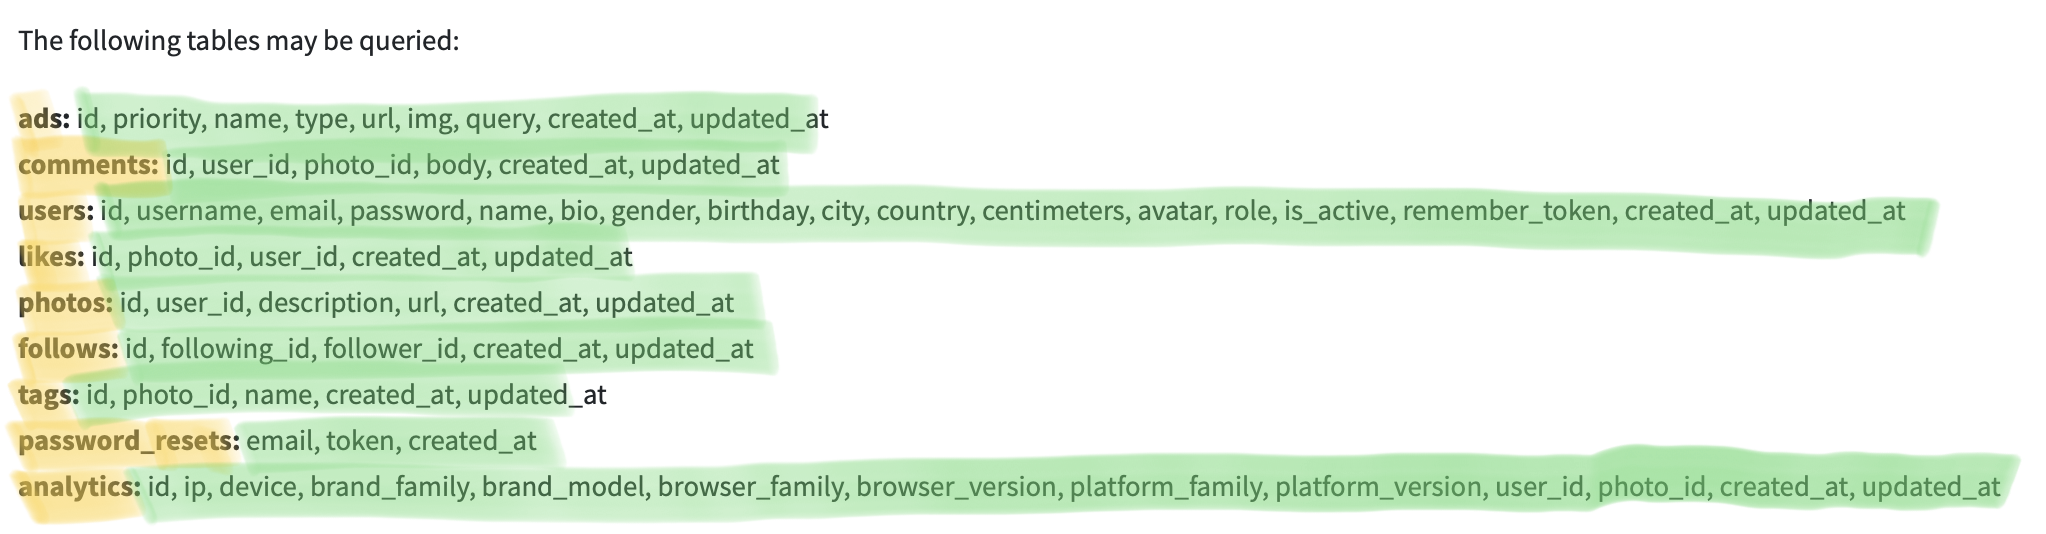
\includegraphics[width=.9\textwidth]{Grundlagen_Info/06_Datenbanken/Figures/instahub-tables}
  %   \caption{Die Tabellen von InstaHub und deren Attribute}
  %   \label{fig:tables-instahub}
  % \end{figure}

Geben Sie in die Eingabezeile von InstaHub den folgenden Befehl ein:

\begin{lstlisting}
SELECT *
FROM users
\end{lstlisting}

Mit diesem Befehl wählen wir alle Spalten (\lstinline|*|) der Tabelle \lstinline|users| aus.
Sie sollten nun die gesamte Tabelle \texttt{users} sehen.
\end{myexample}

\begin{myexercise}
  Geben Sie alle Benutzernamen (\texttt{username}) aus \texttt{users} aus.
  \begin{myanswer}
    \begin{lstlisting}
      SELECT username
      FROM users
      \end{lstlisting}
  \end{myanswer}
\end{myexercise}

\begin{myexercise}
  Geben Sie die Benutzernamen (\texttt{username}) und echten Namen (\texttt{name}) aller Einträge aus \texttt{users} aus.
  \begin{myanswer}
    \begin{lstlisting}
      SELECT username, name
      FROM users
    \end{lstlisting}
  \end{myanswer}
\end{myexercise}

\begin{myexercise}
  Geben Sie die Namen und Wohnorte aller Mitglieder aus.
  \begin{myanswer}
    \begin{lstlisting}
      SELECT username, city
      FROM users
    \end{lstlisting}
  \end{myanswer}
\end{myexercise}

\subsubsection*{Selektion mit Filter: \texorpdfstring{\lstinline|WHERE|}{WHERE}}
Fügen wir zu einer \gls{SQL}-Abfrage den Befehl ``\lstinline|WHERE conditions|'' hinzu, können wir das erhaltene Resultat nach gewissen Bedingungen (\texttt{conditions}) filtern.

\begin{myexample}
Geben Sie folgendes Beispiel in Instahub ein:

\begin{lstlisting}
SELECT name, city, gender
FROM users
WHERE gender="male"
\end{lstlisting}
\end{myexample}

Nebst dem Gleich-Zeichen (im obigen Beispiel) stehen folgende Filter-Operatoren zur Verfügung:
\begin{table}[H]
  \centering
  \begin{tabular}{c|l}
    \makecell{\textbf{Operator}                                                                 \\\textbf{in \gls{SQL}}} & \makecell{\textbf{Mathematische}\\\textbf{Bedeutung}} \\\midrule
    \texttt{=}                                    & gleich ($=$)                                \\
    \texttt{<>}                                   & ungleich ($\neq$)                           \\
    \texttt{<}                                    & kleiner als ($<$)                           \\
    \texttt{<=}                                   & kleiner oder gleich ($\leq$)                \\
    \texttt{>}                                    & grösser als ($>$)                           \\
    \texttt{>=}                                   & grösser oder gleich ($\geq$)                \\
    \lstinline|BETWEEN x AND y|        & ein Wert zwischen (inklusive) \texttt{x} und \texttt{y} \\
    \lstinline|IN (wert1, wert2, ...)| & einer von mehreren möglichen Werten         \\
    \lstinline|IS NULL|                & Wert existiert nicht                        \\
  \end{tabular}
\end{table}
Um mehrere Bedingungen miteinander zu verknüpfen, können wir die Befehle \lstinline|AND|, \lstinline|NOT| sowie \lstinline|OR| verwenden.
%TODO: braucht es eine Erklärung zu Klammern für die richtige Verknüpfung von mehreren Bedingungen?

\begin{myexample}\label{myexample:between}
Folgender Code gibt alle Mitglieder aus, die zwischen 172 cm und 174 cm gross sind. Dabei gehören 172 cm und 174 cm selbst ebenfalls dazu (inklusive).

\begin{lstlisting}
SELECT name, centimeters, gender 
FROM users 
WHERE centimeters BETWEEN 172 AND 174 
\end{lstlisting}
\end{myexample}

\begin{myexample}\label{myexample:in}
Folgender Code gibt den Namen und die Stadt aller männlichen Mitglieder aus, die entweder in Leipzig, Berlin oder Hamburg wohnen.

\begin{lstlisting}
SELECT name, city
FROM users 
WHERE gender = "male" AND city IN ("Leipzig", "Berlin", "Hamburg")
\end{lstlisting}
\end{myexample}


\begin{mycaution}
Wie Sie anhand der \cref{myexample:in,myexample:between} sehen, spielt es in SQL eine Rolle, ob  wir nach Zahlen oder nach
  Text filtern: Wenn nach einem Text gefiltert wird, muss dieser in Anführungszeichen stehen (wie z.B.
  \lstinline|"Berlin"| in \cref{myexample:in}). Bei Zahlen dürfen Sie keine Anführungszeichen schreiben (s. z.B. die Zahl
  \lstinline|172| in \cref{myexample:between}).
\end{mycaution}

\lstinline|NULL| ist ein spezielles \gls{SQL}-Wort, welches bedeutet, dass ein Feld leer ist, bzw. keinen
Wert hat. \lstinline|NULL| muss von \enquote{0} unterschieden werden: Beispielsweise könnte die Zahl 0 in einer 
Tabelle über Bankkonten bedeuten, dass jemand 0 Franken auf seinem Konto hat, während der Wert \lstinline|NULL| bedeuten würde, dass keine 
Informationen zum Kontostand vorhanden sind.

\begin{myexample}
  Folgender Code gibt die Namen aller Mitglieder an, die ihre Grösse nicht angegeben haben.
\begin{lstlisting}
SELECT name, centimeters
FROM users 
WHERE centimeters IS NULL
\end{lstlisting}
\end{myexample}


\begin{myexercise}
  Geben Sie die Namen aller weiblichen Mitglieder aus, die zwischen 150 und 155 gross sind.
  \begin{myanswer}
    \begin{lstlisting}
      SELECT name, gender, centimeters
      FROM users
      WHERE gender="female"
      AND centimeters BETWEEN 150 AND 155
    \end{lstlisting}
  \end{myanswer}
\end{myexercise}
\begin{myexercise}
  Zeigen Sie den Namen, das Geburtsdatum sowie die Grössen aller Frauen an, die kleiner oder gleich 160 Zentimeter sind.
  \begin{myanswer}
    \begin{lstlisting}
      SELECT name, birthday, centimeters
      FROM users
      WHERE gender="female"
      AND centimeters <= 160
    \end{lstlisting}
  \end{myanswer}
\end{myexercise}

\subsubsection*{Sortieren: \texorpdfstring{\lstinline|ORDER BY|}{ORDER BY}}

Mit dem Befehl \lstinline|ORDER BY col ASC| oder \lstinline|ORDER BY col DESC| kann das Resultat einer \gls{SQL} -Abfrage nach einer bestimmten Kolonne \lstinline|col| sortiert werden. Mit \lstinline|ASC| wird das Resultat aufsteigend und mit \lstinline|DESC| absteigend sortiert.

\begin{myexample}
Beobachten Sie das Resultat folgender Abfrage:

\begin{lstlisting}
SELECT name, centimeters 
FROM users 
ORDER BY centimeters DESC
\end{lstlisting}
\end{myexample}

\begin{myexercise}
  Geben Sie alle Benutzernamen in sortierter Reihenfolge aus (a $\rightarrow$ z).
  \begin{myanswer}
    \begin{lstlisting}
SELECT username
FROM users
ORDER BY username ASC
\end{lstlisting}
  \end{myanswer}
\end{myexercise}

\begin{mysubmission}
  Bearbeiten Sie auf Moodle die ``Übung 1: Einfache SQL Abfragen'' und geben Sie am Schluss ab.
\end{mysubmission}

\subsection{Neue Tabellen und Verknüpfungen}
\subsubsection{1:n-Verknüpfung}
Die Verwaltung der Nutzer Ihrer neuen Social-Media-Plattform ist bereit. Nun sollen die Nutzer auch Bilder hochladen können. Die Frage ist: Wie können Bilder in der Datenbank gespeichert und mit dem entsprechenden user verknüpft werden?

Eine erste Idee könnte sein, dass man der Tabelle \enquote{users} ein zusätzliches Attribut \enquote{url} mit der Adresse des Bildes hinzufügt.

Wenn jemand aber mehr als ein Bild hochlädt, sähe die Tabelle wie in \Cref{fig:photoAlsSpalte} (wobei zur besseren Übersicht nur einige wenige Zeilen und Spalten angezeigt werden)
\begin{center}
  \begin{figure}[ht!]
    % \includegraphics[width = 0.6 \textwidth]{Grundlagen_Info/06_Datenbanken/Figures/redundanz.png}
  \end{figure}
  \label{fig:photoAlsSpalte}
\end{center}

Das ist zwar eine funktionierende Möglichkeit, mit ihr kommen aber zwei wesentliche Probleme:
\begin{itemize}
  \item Diese Lösung benötigt viel Speicherplatz: Für jedes Bild wird ein neuer Eintrag in der Tabelle users erstellt, bei dem alle Benutzerangaben wie id, username, password, usw. kopiert werden.
  \item Diese Lösung ist schwer zu verwalten: Stellen Sie sich vor, dass ein Benutzer seine E-Mail-Adresse aktualisiert. Bei dieser Lösung muss die neue Adresse an vielen stellen der Tabelle verändert werden.
\end{itemize}

Wenn in einer Tabelle die gleiche Information mehrfach vorkommt, spricht man von \textbf{Redundanzen}. Ein wichtiges Ziel der Verwaltung von Informationen in Datenbanken ist es, Redundanzen zu vermeiden.

Anstatt die Bilder in die bestehende Tabelle einzufügen, wird eine neue Tabelle \enquote{photos} erstellt, die dann mit der Tabelle \enquote{users} verknüpft wird. Die neue Tabelle hat die Attribute \textit{id, user\_id, description, url, created\_at, updated\_at}. 


Zur besseren Übersicht führen wir sogenannte Tabellenkarten ein. In diesen werden der Tabellenname und die Attribute angegeben. Für die bereits bekannten Tabellen sieht das so aus:

\begin{table}[h!]
  \centering
  \begin{tabular}{m{6cm} m{4cm}}
      % Users table
      \begin{tabular}{|l|}
      \hline\textbf{users}
      \\ \hline
      id \\
      username \\
      email \\
      password \\
      name \\
      bio \\
      gender \\
      birthday \\
      city \\
      country \\
      centimeters \\
      avatar \\
      role \\
      is\_active \\
      remember\_token \\
      created\_at \\
      updated\_at \\ \hline
      \end{tabular}
      &
      % Photos table
      \begin{tabular}{|l|}
      \hline
      \textbf{photos} \\ \hline
      id \\
      user\_id \\
      description \\
      url \\
      created\_at \\
      updated\_at \\ \hline
      \end{tabular}
  \end{tabular}
\end{table}



Zwischen den Tabellen gibt es eine Verknüpfung. Ein Nutzer kann viele Bilder besitzen. Jedes Bild gehört aber immer genau einem Benutzer. Eine solche Beziehung zwischen zwei Tabellen nennt man eine \textbf{1:n-Verknüpfung} (Ein (1) User kann viele (n) Bilder hochladen).

Die Verknüpfung der Tabellen in einer Datenbank wird häufig grafisch durch ein \acrfull{ERM} dargestellt.

Ein \acrfull{ERM} ist eine abstrakte Darstellung der Tabellen (Entities), die in einer Datenbank angelegt sind, sowie der Beziehungen (Relationships) zwischen den Tabellen. Jede Tabelle kann mehrere Kolonnen (= Attribute) haben.

Das \gls{ERM} unserer Datenbank sieht im Moment wie folgt aus:


% Wenn man eine Datenbank erstellt, kann es nützlich sein, zuerst ein \gls{ERM} aufzuzeichnen, um sich zu überlegen, welche Tabellen es braucht.

% Das \gls{ERM} des sozialen Netzwerks InstaHub ist in \cref{fig:erm-instahub} abgebildet. \cref{fig:erm-components} zeigt die Darstellung der Komponenten eines ERM in der sogenannten Chen-Notation.

\begin{figure}[H]
  \centering
  \begin{tikzpicture}[auto]
    % Nodes
    \node[entity] (user) at (0,0) {users};
    \node[entity] (photo) at (5,0) {photos};
    \node[relationship] (owns) at (2.5,0) {owns};
  

    % Edges
    \draw (user) -- (owns) node[midway, above] {1};
    \draw (owns) -- (photo) node[midway, above] {n};
    
  \end{tikzpicture}
  \caption{\gls{ERM} von Instahub - Version 1}
  \label{fig:erm-instahub-v1}
\end{figure}

% \begin{figure}[H]
%   \centering
%   \begin{tikzpicture}[node distance=1cm]

%     % Entity
%     \node[entity] (entity1) {Entity};
%     \node[attribute] (attr1) [above left=of entity1] {Attribute} edge (entity1);
%     \node[attribute] (attr2) [below left=of entity1] {Attribute} edge (entity1);

%     % Relationship
%     \node[relationship] (rel1) [right=3cm of entity1] {Relationship} edge node[auto,swap] {n} (entity1);
%     \node[entity] (entity2) [right=3cm of rel1] {Entity} edge node[auto,swap] {m} (rel1);
%     \node[attribute] (attr3) [above=of rel1] {Attribute} edge (rel1);

%     % Legend
%     \node[draw,thick,fit=(entity1) (attr1) (attr2),inner sep=0.5cm, rounded corners, dotted, red] (box1) {};
%     \node[anchor=south, red] at (box1.north) {Tabellen (\textit{Entities}) und Attribute};

%     \node[draw,thick,fit=(rel1) (entity2) (attr3),inner sep=0.5cm, rounded corners, dotted, blue] (box2) {};
%     \node[anchor=south, blue] at (box2.north) {Beziehungen (\textit{Relationships})};

%   \end{tikzpicture}
%   \caption{\gls{ERM}-Komponenten in der sogenannten Chen-Notation}
%   \label{fig:erm-components}
% \end{figure}

Die Tabellen, werden als Rechtecke angegeben. Beziehungen stellen ``Verknüpfungen'' zwischen verschiedenen Tabellen dar und sind meist als Rhombus dargestellt. Manchmal werden auch die Attribute als Ovale angegeben. Weil die Tabelle users viele Attribute umfasst, sind diese in \cref{fig:erm-instahub-v1} einfachheitshalber nicht angegeben.

\subsubsection*{Wie wird die 1:n-Verknüpfung der Tabellen realisiert?}

Für die Verknüpfung der Tabellen in der Datenbank spielen die \textbf{Primärschlüssel} eine wichtige Rolle. Jede Tabelle in einer Datenbank besitzt einen solchen Primärschlüssel. Dabei handelt es sich um \textbf{einen oder mehreren Attributen, die jeden Datensatz eindeutig identifizieren}.

In der Tabelle \enquote{users} ist der Primärschlüssel das Attribut \emph{id}. 

Wie in \cref{subsec:tables} diskutiert wurde, besitzen Tabellen häufig sogenannte Primärschlüssel (en. \textit{primary keys}). Dabei handelt es sich um \textbf{einen oder mehreren Attributen, die jeden Datensatz eindeutig identifizieren}. 

Die Tabelle \enquote{users} beispielsweise verwendet den Primärschlüssel \underline{id} (blaue Kolonne, Titel unterstrichen, hervorgehoben mit dem Symbol \emoji{key}). 

\begin{table}[H]
\centering
\begin{tabular}{a|l|l}
\emoji{key} \underline{id} & name   & ... \\\midrule
1  & Niclas Schweizer  & ...  \\
2  & Rafael Probst & ...  \\
3  & Luis Krüger  & ...\\
... & ... & ... 
\end{tabular}
\caption{Beispiel-Tabelle: ``users''}
\label{table:users-primaryKey}
\end{table}

Datenbanken sind so programmiert, dass jeder Datensatz in der Primärschlüssel-Spalte(n) einen Eintrag haben muss und sich diese Einträge paarweise unterscheiden. Der Primärschlüssel dient in erster Linie dazu, einen Datensatz (in diesem Fall eine Person) eindeutig zu identifizieren. Weshalb ist das nötig? 

Zwei Hauptgründe seien angegeben:

\begin{itemize}
\item \textbf{Eindeutigkeit}: Es könnte sein, dass zwei Personen gleich heissen. In diesem Fall ist es hilfreich, eine eindeutige Identifikationsnummer (oder einen eindeutigen Text) zu haben, um Information zu genau \textit{einer} der beiden Personen abfragen zu können.
\item \textbf{Dauerhaftigkeit}: Es könnte sein, dass eine Person den Namen wechselt. In diesem Fall möchte man eine eindeutige Identifikationsnummer haben, damit die Informationen zu den Personen wie etwa Fotos oder Kommentare weiterhin eindeutig zur selben Person gehören (und abgefragt werden können).
\end{itemize}

Aus eben diesen Gründen hat jede Person in der Schweiz übrigens eine \href{https://www.bsv.admin.ch/bsv/de/home/sozialversicherungen/ahv/grundlagen-gesetze/ahv-nummer.html}{AHV-Nummer} : \begin{quote}
  ``Die 13-stellige AHV-Nummer ist völlig anonym, zufallsgeneriert und nicht sprechend. Sie wird nur einmal vergeben und bleibt ein Leben lang unverändert, auch wenn der Zivilstand - etwa durch Heirat - ändert.''
\end{quote}


Nebst Primärschlüsseln können Tabellen auch sogenannte Fremdschlüssel (en. \textit{foreign keys}) besitzen, die sich auf Primärschlüssel von anderen Tabellen beziehen. Dies erlaubt, Informationen aus mehreren Tabellen zu kombinieren. Bei den beiden Tabellen \enquote{users} und \enquote{photos} sieht das so aus: (\cref{table:users-2}, \cref{table:photos-2}).

\begin{minipage}{.38\textwidth}
\centering

\begin{table}[H]
\centering
\begin{tabular}{a|l}
  \tikzmarknode{pkey}{\emoji{key}} \underline{id} & name    \\\midrule
\tikzmarknode{1t}{1}  & Niclas Schweizer    \\
\tikzmarknode{2t}{2}  & Rafael Probst   \\
\tikzmarknode{3t}{3}  & Luis Krüger  \\
... & ...
\end{tabular}
\caption{Tabelle ``\textbf{users}''}
\label{table:users-2}
\end{table}
\end{minipage}
\begin{minipage}{.58\textwidth}
\centering
\begin{table}[H]
\centering
\begin{tabular}{a|l|l}
  \emoji{key} \underline{id} &\tikzmarknode{fkey}{\faKey \dashuline{user\_id}} & url \\\midrule
  \dots & \dots & \dots \\
41 & \tikzmarknode{1o}{1}   & island-eb32b30d2c\_960.jpg   \\
42& \tikzmarknode{1o1}{1}   & amusement-eb31b40921\_960.jpg    \\
43& \tikzmarknode{2o}{2}    & teacup-eb36b30a2f\_960.jpg  \\
\dots & \dots& \dots
\end{tabular}
\begin{tikzpicture}[overlay,remember picture]
% title
 \draw[red,-stealth] (fkey) to[bend right] (pkey);
% values
  \draw[red,-stealth] (1o) -- (1t);
  \draw[red,-stealth] (1o1) -- (1t);
  \draw[red,-stealth] (2o) -- (2t);
\end{tikzpicture}
\caption{Tabelle ``\textbf{photos}''}
\label{table:photos-2}
\end{table}
\end{minipage}

Die Tabelle ``photos'' hat nicht nur einen Primärschlüssel \texttt{id}, sondern auch einen Fremdschlüssel \texttt{user\_id} (unterbrochen unterstrichen und hervorgehoben mit dem Symbol \faKey), der auf den Primärschlüssel der Tabelle ``users'' verweist. 

Die Datenbank von Instahub ist ausserdem so konzipiert, dass jedes Foto durch mehrere \enquote{Tags} beschrieben werden kann. Umgekehrt gehört jeder Tag zu genau einem\footnote{Man könnte darüber streiten, es sinnvoll ist, das Tags nicht zu mehreren Fotos gehören können. Bei Instahub ist das aber so festgelegt.} Foto. Das ERM sieht dann so aus:

\begin{figure}[H]
  \centering
  \begin{tikzpicture}[auto]
    % Nodes
    \node[entity] (user) at (0,0) {users};
    \node[entity] (photo) at (5,0) {photos};
    \node[relationship] (owns) at (2.5,0) {owns};
    \node[entity] (tag) at (10,0) {tags};
    \node[relationship] (has) at (7.5,0) {has};
  

    % Edges
    \draw (user) -- (owns) node[midway, above] {1};
    \draw (owns) -- (photo) node[midway, above] {n};
    \draw (photo) -- (has) node[midway, above] {1};
    \draw (has) -- (tag) node[midway, above] {n};
    
  \end{tikzpicture}
  \caption{\gls{ERM} von Instahub - Version 2}
  \label{fig:erm-instahub-v2}
\end{figure}

Wobei die Tabelle \enquote{tags} die folgenden Attribute hat (Primärschlüssel unterstrichen, Fremdschlüssel unterbrochen unterstrichen)
\begin{center}
  \begin{tabular}{|l|}
    \hline
    \textbf{tags} \\ \hline
    \uline{id} \\
    \dashuline{photo\_id} \\
    name \\
    created\_at \\
    updated\_at \\ \hline
    \end{tabular}
\end{center}

In den folgenden Aufgaben wollen wir unsere Social-Media-Plattform um die Tabellen \enquote{photos} und \enquote{users} erweitern. Dazu verwenden wir den SQL-Befehl \lstinline|CREATE TABLE|. Dieser ist wie folgt aufgebaut:
\begin{lstlisting}
  CREATE TABLE Tabellenname (
    Spalte1   Datentyp1   weitereEigenschaftenSpalte1,
    Spalte2   Datentyp2   weitereEigenschaftenSpalte2,
    Spalte3   Datentyp3   weitereEigenschaftenSpalte3,
    ...       ...         ...
  )
\end{lstlisting}

\begin{myexercise}[Tabelle photos anlegen]
  \begin{lstlisting}
    CREATE TABLE `photos` (
      `id` int(10) UNSIGNED NOT NULL AUTO_INCREMENT,
      `user_id` int(10) UNSIGNED NOT NULL,
      `description` varchar(191) NOT NULL,
      `url` varchar(191) NOT NULL,
      `created_at` timestamp NULL DEFAULT NULL,
      `updated_at` timestamp NULL DEFAULT NULL,
      PRIMARY KEY (`id`),
      FOREIGN KEY (`user_id`) REFERENCES `users`(`id`) ON DELETE CASCADE
    )
  \end{lstlisting}
  \begin{enumerate}
    \item Versuchen Sie den Befehl oben nachzuvollziehen: Welche Spalten wird die neue Tabelle umfassen? Welches ist der Primärschlüssel der neuen Tabelle? Welches der Fremdschlüssel? Mit welcher Spalte welcher Tabelle ist der Fremdschlüssel verbunden?
    \item    Loggen Sie sich als admin bei Ihrem Instahub ein und navigieren Sie zur Datenbank-Administration.
    \begin{figure}[H]
      \centering
      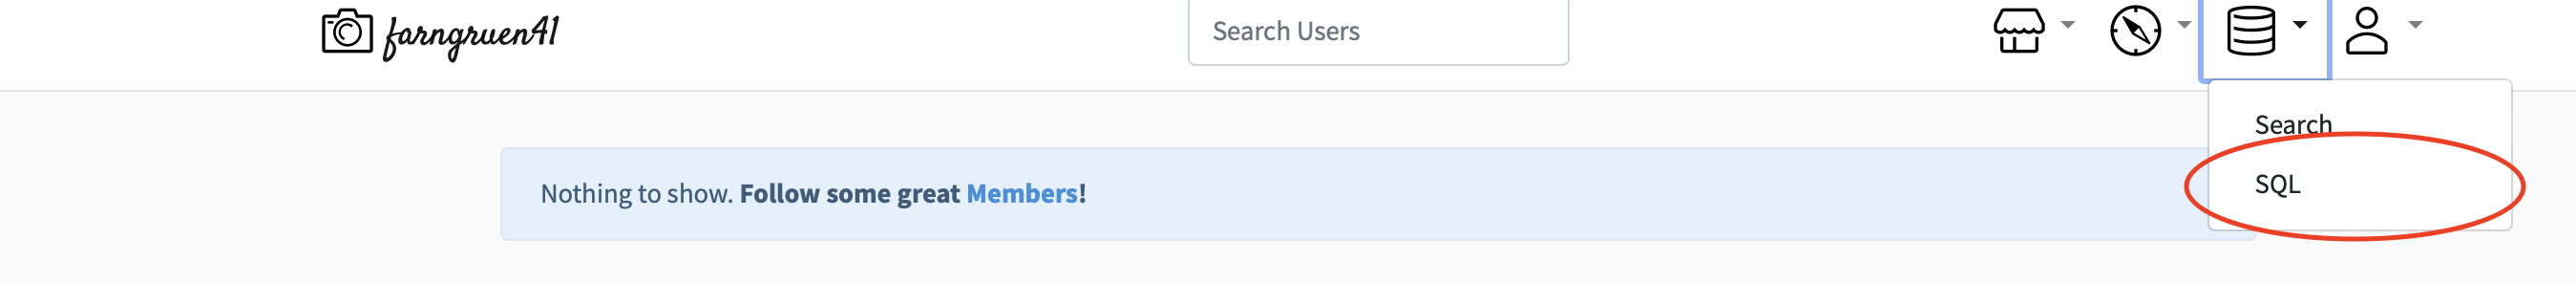
\includegraphics[width=.9\textwidth]{Grundlagen_Info/06_Datenbanken/Figures/instahub-SQL}
    \end{figure}
    \item Kopieren Sie den Befehl oben in die Eingabezeile und führen Sie ihn aus. Unter \enquote{Folgende einzelne Tabellen können abgefragt werden} sollte nun die Tabelle \enquote{photos} aufgeführt sein. (Eventuell müssen Sie die Seite zuerst neu laden)
    \item Testen Sie, ob Sie nun neu ein Foto hochladen können: Klicken Sie auf Ihr Nutzersymbol (rechts oben im Fenster) und wählen Sie \enquote{Hochladen} (Eventuell müssen Sie die Seite zuerst neu laden, damit die Option verfügbar ist). Laden Sie ein Bild hoch (nichts persönliches).
    \item Für das Bild mussten Sie zwingend eine Beschreibung angeben. Welcher Teil des Befehls oben hatte diese Auswirkung?
    \item Gehen Sie zurück zur Datenbank-Verwaltung und lassen Sie sich alle Inhalte (\lstinline|SELECT *|) der Tabelle \enquote{photos} anzeigen. 
    \item Löschen Sie Ihr Bild wieder mit dem Befehl \lstinline|DELETE FROM photos WHERE id = 1|. Kontrollieren Sie, dass die Datenbank leer ist. (Falls noch etwas darin ist, können Sie den gesamten Inhalt der Tabelle löschen mit \lstinline|DELETE FROM photos|).
  \end{enumerate}

  Die Nutzer Ihrer Plattform haben unterdessen auch gemerkt, dass man Fotos hochladen kann, was sie fleissig tun. Simulieren Sie ihre Aktivität, indem Sie den folgenden \href{https://wi-wissen.github.io/instahub-doc-de/sql/photos.sql}{Befehl zum Füllen der Tabelle} \enquote{photos} runterladen, mit einem Text-Editor öffnen, per Copy/Paste in die Eingabezeile übertragen und schliesslich ausführen.

  Wenn Sie möchten, können Sie die Bilder Ihrer Nutzer nun anschauen\dots
\end{myexercise}



\begin{myexercise}[Tabelle tags anlegen]
  \begin{lstlisting}
    CREATE TABLE `tags` (
      `id` int(10) UNSIGNED NOT NULL AUTO_INCREMENT,
      `photo_id` int(10) UNSIGNED NOT NULL,
      `name` varchar(191) NOT NULL,
      `created_at` timestamp NULL DEFAULT NULL,
      `updated_at` timestamp NULL DEFAULT NULL,
      PRIMARY KEY (id),
      FOREIGN KEY (`photo_id`) REFERENCES `photos`(`id`) ON DELETE CASCADE
    )
  \end{lstlisting}
  \begin{enumerate}
    \item Versuchen Sie den Befehl oben nachzuvollziehen: Welche Spalten wird die neue Tabelle umfassen? Welches ist der Primärschlüssel der neuen Tabelle? Welches der Fremdschlüssel? Mit welcher Spalte welcher Tabelle ist der Fremdschlüssel verbunden?
    \item  Kopieren Sie den Befehl in die SQL-Eingabezeile Ihres Instahubs und führen Sie ihn aus. 
    \item Um aus den bestehenden Bildbeschreibungen die Tags zu extrahieren, können Sie folgende
    Webadresse aufrufen: \url{https://[meinefarbeXX].instahub.org/dba/updateTags}
    \item Überprüfen Sie, ob die Tabelle \enquote{tags} gefüllt wurde, indem Sie mit einem entsprechenden SQL-Befehl die Inhalte anzeigen lassen.
  \end{enumerate}

\end{myexercise}


\subsubsection{n:m Verknüpfung zwischen Tabellen}
Die Nutzer Ihrer Social-Media-Plattform sind nun in der Lage, Bilder hochzuladen und mit Tags zu versehen. Damit es zu einer ersten Interaktion zwischen den Nutzern kommt, sollen diese auch Bilder liken konnen.

Konkret soll jeder Nutzer mehrere Bilder liken können und jedes Bild soll (möglicherweise) Likes von mehreren unterschiedlichen Usern erhalten können. Diese Art der Beziehung zwischen den beiden Tabellen \enquote{users} und \enquote{photos} bezeichnet man als eine \textbf{n:m Verknüpfung}. (Ein Bild kann mehrere (n) Likes erhalten und ein User kann mehrere (m) Bilder liken.)

Das \gls{ERM} sieht dann wie folgt aus:
\begin{figure}[H]
  \centering
  \begin{tikzpicture}[auto]
    % Nodes
    \node[entity] (user) at (0,0) {users};
    \node[entity] (photo) at (5,0) {photos};
    \node[relationship] (owns) at (2.5,0) {owns};
    \node[entity] (tag) at (10,0) {tags};
    \node[relationship] (has) at (7.5,0) {has};
    \node[relationship] (likes) at (2.5,-2.5) {likes};
  

    % Edges
    \draw (user) -- (owns) node[midway, above] {1};
    \draw (owns) -- (photo) node[midway, above] {n};
    \draw (photo) -- (has) node[midway, above] {1};
    \draw (has) -- (tag) node[midway, above] {n};
    \draw (user) -- (likes) node[midway, left] {n};
    \draw (likes) -- (photo) node[midway, right] {m};
    
  \end{tikzpicture}
  \caption{\gls{ERM} von Instahub - Version 3}
  \label{fig:erm-instahub-v3}
\end{figure}
  
Eine solche Verknüpfung von zwei Tabellen wird mit einer Zwischentabelle realisiert. Diese enthält zwei Fremdschlüsseln: einen der auf den Primärschlüssel der ersten Tabelle verweist und einen auf jenen der zweiten Tabelle.

\begin{table}[H]
  \centering
  \begin{tabular}{l|l}
  \dashuline{user\_id} &  \dashuline{photo\_id}   \\
  \midrule
  11  & 32 \\
  11  & 42  \\
  12  & 42   \\ 
  \end{tabular}
  \caption{Beispiel-Tabelle: ``likes''}
  \label{table:likes}
  \end{table}

In diesem Beispiel hat der*die Benutzer*in mit der id 11 die Fotos Nr. 32 und Nr. 42 geliked. Das Bild Nr. 42 hat ausserdem einen Like von User Nr. 12 erhalten.

Eine solche Tabelle würde im Prinzip schon ausreichen, um die n:m Verknüpfung von \enquote{users} und \enquote{photos} zu verwicklichen. In Instahub wurden in der Tabelle \enquote{likes} allerdings weitere Informationen darüber abgelegt, wann der Like vergeben wurde. Die Tabelle \enquote{likes}, wie sie in Instahub realisiert wurde, hat die folgenden Atribute:

\begin{center}
  \begin{tabular}{|l|}
    \hline
    \textbf{likes} \\ \hline
    \uline{id} \\
    \dashuline{photo\_id} \\
    \dashuline{user\_id} \\
    created\_at \\
    updated\_at \\ \hline
    \end{tabular}
\end{center}


\begin{myexercise}[Tabelle \enquote{likes} erstellen]
  \begin{lstlisting}
    CREATE TABLE `likes` (
      `id` int(10) UNSIGNED NOT NULL AUTO_INCREMENT,
      `photo_id` int(10) UNSIGNED NOT NULL,
      `user_id` int(10) UNSIGNED NOT NULL,
      `created_at` timestamp NULL DEFAULT NULL,
      `updated_at` timestamp NULL DEFAULT NULL,
      PRIMARY KEY (`id`),
      FOREIGN KEY (`photo_id`) REFERENCES `photos`(`id`) ON DELETE CASCADE,
      FOREIGN KEY (`user_id`) REFERENCES `users`(`id`) ON DELETE CASCADE
      )
  \end{lstlisting}
  \begin{enumerate}
    \item Versuchen Sie den Befehl oben nachzuvollziehen.
    \item Kopieren Sie den Befehl in die SQL-Eingabezeile Ihres Instahubs und führen Sie ihn aus. 
    \item Simulieren Sie die Aktivität Ihrer Nutzer, indem Sie den folgenden \href{https://wi-wissen.github.io/instahub-doc-de/sql/likes.sql}{Befehl zum Füllen der Tabelle likes} \enquote{photos} runterladen, mit einem Text-Editor öffnen, per Copy/Paste in die Eingabezeile übertragen und schliesslich ausführen.
  \end{enumerate}

\end{myexercise}

Analog zur Tabelle \enquote{likes} gibt es in InstaHub zwei weitere Hilfstabellen \enquote{comments} und \enquote{follows}, um die n:m Verknüpfung der Tabellen \enquote{users - photos} und \enquote{users - users} abzubilden.

Das vollständige \gls{ERM} von Instahub ist:

\begin{figure}[H]
  \centering
  \begin{tikzpicture}[auto]
    % Nodes
    \node[entity] (user) at (0,0) {users};
    \node[relationship] (follows) at (-4,0) {follows};
    \node[relationship] (owns) at (2.5,0) {owns};
    \node[entity] (photo) at (5,0) {photos};
    \node[relationship] (has) at (7,0) {has};ff
    \node[entity] (tag) at (9,0) {tags};
    \node[relationship] (comments) at (2.5,2.5) {comments};
    \node[relationship] (likes) at (2.5,-2.5) {likes};
    % \node[relationship] (haspw) at (0,-2) {has};
    % \node[entity] (pwreset) at (-4,-2) {password\_resets};

    % Edges
    \draw (user) -- (follows) node[midway, above] {m};
    \draw (follows) -- (user) node[midway, below] {n};
    \draw (user) -- (owns) node[midway, above] {1};
    \draw (owns) -- (photo) node[midway, above] {n};
    \draw (photo) -- (has) node[midway, above] {1};
    \draw (has) -- (tag) node[midway, above] {n};
    \draw (user) -- (comments) node[midway, above] {n};
    \draw (comments) -- (photo) node[midway, above] {m};
    \draw (user) -- (likes) node[midway, left] {n};
    \draw (likes) -- (photo) node[midway, right] {m};
    % \draw (user) -- (haspw) node[midway, left] {1};
    % \draw (haspw) -- (pwreset) node[midway, above] {n};
  \end{tikzpicture}
  \caption{\gls{ERM} von InstaHub}
  \label{fig:erm-instahub}
\end{figure}

\begin{myexercise}[Tabellen \enquote{comments} erstellen]
  \begin{lstlisting}
    CREATE TABLE `comments` (
      `id` int(10) UNSIGNED NOT NULL AUTO_INCREMENT,
      `user_id` int(10) UNSIGNED NOT NULL,
      `photo_id` int(10) UNSIGNED NOT NULL,
      `body` varchar(191) NOT NULL,
      `created_at` timestamp NULL DEFAULT NULL,
      `updated_at` timestamp NULL DEFAULT NULL,
      PRIMARY KEY (`id`),
      FOREIGN KEY (`photo_id`) REFERENCES `photos`(`id`) ON DELETE CASCADE,
      FOREIGN KEY (`user_id`) REFERENCES `users`(`id`) ON DELETE CASCADE
    )
  \end{lstlisting}
  \begin{enumerate}
    \item Kopieren Sie den Befehl in die SQL-Eingabezeile Ihres Instahubs und führen Sie ihn aus. 
    \item Simulieren Sie die Aktivität Ihrer Nutzer, indem Sie den folgenden \href{https://wi-wissen.github.io/instahub-doc-de/sql/comments.sql}{Befehl zum Füllen der Tabelle comments} \enquote{photos} runterladen, mit einem Text-Editor öffnen, per Copy/Paste in die Eingabezeile übertragen und schliesslich ausführen.
  \end{enumerate}

\end{myexercise}

\begin{myexercise}[Tabellen \enquote{follows} erstellen]
  \begin{lstlisting}
    CREATE TABLE `follows` (
      `id` int(10) UNSIGNED NOT NULL AUTO_INCREMENT,
      `following_id` int(10) UNSIGNED NOT NULL,
      `follower_id` int(10) UNSIGNED NOT NULL,
      `created_at` timestamp NULL DEFAULT NULL,
      `updated_at` timestamp NULL DEFAULT NULL,
      PRIMARY KEY (`id`),
      FOREIGN KEY (`following_id`) REFERENCES `users`(`id`) ON DELETE CASCADE,
      FOREIGN KEY (`follower_id`) REFERENCES `users`(`id`) ON DELETE CASCADE
    )
  \end{lstlisting}
  \begin{enumerate}
    \item Kopieren Sie den Befehl in die SQL-Eingabezeile Ihres Instahubs und führen Sie ihn aus. 
    \item Simulieren Sie die Aktivität Ihrer Nutzer, indem Sie den folgenden \href{https://wi-wissen.github.io/instahub-doc-de/sql/follows.sql}{Befehl zum Füllen der Tabelle follows} \enquote{photos} runterladen, mit einem Text-Editor öffnen, per Copy/Paste in die Eingabezeile übertragen und schliesslich ausführen.
  \end{enumerate}
  Gratulation: Ihre Social-Media-Plattform ist nun voll funktionsfähig!
\end{myexercise}

\begin{myexercise}
  [Aufteilen von Informationen auf verschiedene Tabellen]
  Für die Organisation der Skilager führt die Schule eine Liste mit mehreren hundert Einträgen. Der Anfang der Liste sieht wie folgt aus:

  \begin{tabular}{l|l|l}
    Name	& Klasse&	Allergen \\ \hline 
    Alice	&1a	&Nüsse \\
    Bob	&1a	&Gluten \\
    Charly	&2b	&Nüsse, Laktose \\
    Deborah	&1c&	 \\
    Elisa	&4c	&Laktose \\
    Fiona	&2b	& \\
    ...	&...	&...
  \end{tabular}


Diese Liste soll in eine Datenbank umgewandelt werden, um Redundanzen zu vermeiden.

Erklären Sie, wie diese Datenbank aufgebaut sein wird:

\begin{itemize}
  \item Welche Tabellen und Zwischentabellen umfasst die Datenbank?
  \item Welche Attribute müssen in den einzelnen Tabellen vorkommen?
  \item Welches sind die Primär- und gegebenenfalls die Fremdschlüssel in den einzelnen Tabellen?
  \item Zeichnen Sie das dazugehörige ERM-Diagramm.
  \item Geben Sie die einzelnen Tabellen konkret an und füllen Sie sie mit den Daten aus der obigen Liste.
\end{itemize}
\end{myexercise}


\begin{mysubmission}
  Bearbeiten Sie auf Moodle die ``Übung 2: Tabellen Erstellen und Verknüpfen'' und geben Sie am Schluss ab.
\end{mysubmission}


















\subsection{Abfragen über mehrere Tabellen}

Wenn man sich nun zum Beispiel für alle Bilder interessiert, die von Personen aus München hochgeladen wurden, so liegen diese Informationen in zwei unterschiedlichen (aber verknüpften) Tabellen \enquote{users} und \enquote{photos}. Für solche Abfragen muss man die Tabellen zuerst verschmelzen. Dazu dient der SQL-Befehl \lstinline|INNER JOIN|.

Die Syntax eines \lstinline|INNER JOIN|-, oder auch einfach \lstinline|JOIN|-Befehls sieht wie folgt aus:

\begin{lstlisting}
SELECT kolonne1, kolonne2, ...
FROM tabelle1
INNER JOIN tabelle2
ON tabelle1.kolonne_id1 = tabelle2.kolonne_id2
\end{lstlisting}
Hier verbinden wir zwei Tabellen, indem wir zwei Kolonnen \texttt{kolonne\_id1} und \texttt{kolonne\_id2}, die derselben Information entsprechen (beispielsweise die user-ID), miteinander abgleichen. Beim \lstinline|INNER JOIN| werden nur die Zeilen aus \texttt{tabelle1} retourniert, für die es einen entsprechenden Wert in \texttt{kolonne\_id2} in \texttt{tabelle2} gibt. Alle Werte in \texttt{tabelle1} die mit keinem Wert in \texttt{tabelle2} überschneiden, sowie umgekehrt, tauchen nicht im Resultat auf.

\begin{myexample}
  Folgender Code gibt die ids aller Bilder von user Mika Kaufmann zurück
  \begin{lstlisting}
  SELECT photos.id
  FROM photos INNER JOIN users 
  ON photos.user_id = users.id 
  WHERE name = "Mika Kaufmann"
  \end{lstlisting}
  
  Wie Sie sehen, kann es hilfreich sein, im \lstinline|SELECT|-Ausdruck explizit die Tabelle zu nennen, von welcher eine bestimmt Kolonne stammt.
  \end{myexample}

  Einige Informationen sind sogar über drei Tabellen verteilt. So zum Beispiel die Beschreibung aller Bilder, die von Mika Kaufmann geliked wurden. Dazu muss man die Tabellen \enquote{users, photos} und die Hilfstabelle \enquote{likes} schrittweise verknüpfen:

  \begin{myexample}
    Folgender Code gibt die Beschreibung aller Bilder aus, die von Mika Kaufmann geliked werden:
    \begin{lstlisting}
      SELECT photos.description
      FROM photos INNER JOIN (
        users INNER JOIN likes
        ON likes.user_id = users.id
        )
      ON likes.photo_id = photos.id 
      WHERE name = "Mika Kaufmann"
    \end{lstlisting}
    
    In den Klammern werden zuerst die beiden Tabellen \enquote{users} und \enquote{likes} über den Fremdschlüssel \enquote{likes.user\_id} verschmelzt. Die resultierende Tabelle wird schliesslich mit der tabelle \enquote{photos} über den Fremdschlüssel \enquote{likes.photo\_id} verbunden.
    \end{myexample}

  % \begin{mysummary}
  %   Redundanzen in den Informationen verschwenden Speicherplatz und erschweren die Verwaltung.
  %   \begin{itemize}
  %     \item Zur Vermeidung von Redundanzen werden Informationen in einer Datenbank in separaten Tabellen verwaltet.
  %     \item Jede Tabelle hat einen Primärschlüssel, mit dem man die Datensätze eindeutig identifizieren kann.
  %     \item Je zwei Tabellen in einer Datenbank können miteinander verknüpft werden.
  %     \item Wird ein Datensatz der einen Tabelle mit mehreren Datensätzen einer anderen Tabelle in Verbindungen gebracht spricht man von einer \textbf{1:n-Verknüpfung}
  %     \item Eine 1:n-Verknüpfung wird in der Datenbank so realisiert, dass die Tabelle auf der n-Seite einen sogenannten Fremdschlüssel besitzt, der sich auf den Primärschlüssel der Tabelle auf der 1-Seite bezieht.
  %   \end{itemize}
  %   \end{mysummary}

  \begin{mysubmission}
    Bearbeiten Sie auf Moodle die ``Übung 3: SQL-Abfragen über mehrere Tabellen'' und geben Sie am Schluss ab.
  \end{mysubmission}
  
  
   


